\section{迭代的几何运算}
\label{sec:mfo-operations}

现在假定当前点$\bm{x}$处已经算出一个切向候选步$\bm{v}\in T_{\bm{x}}M$。欧氏空间里接下来的事情都是加减法，到了流形上有三件事要重新回答：走完之后怎样回到集合上，怎样评价这一步好不好，历史上的向量在新点怎样使用。

图~\ref{fig:mfo-iteration-loop}是后面所有算法共用的循环。切向候选步由各节的方法给出，其余三个方框分别由下面三小节回答。这里只讨论能在计算机上执行的运算，切空间、联络和指数映射的定义仍以卷四为准。

\begin{BookInlineFigure}
 \centering
 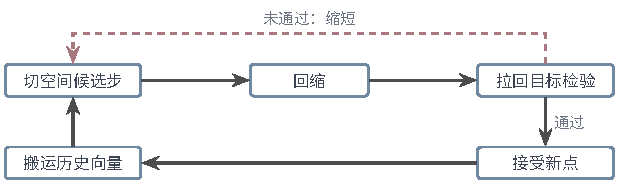
\includegraphics[width=104.7mm]{figures/05-optimization/06-constrained-optimization/tikz/mfo-iteration-loop/figure.pdf}
 \caption{流形优化的一轮迭代。切空间里产生候选步，回缩把它变成流形上的候选点，再用拉回后的目标判断是否接受；接受后把需要保留的历史向量搬到新点的切空间。红色虚线表示判断未通过时缩短步长或半径。}
 \label{fig:mfo-iteration-loop}
\end{BookInlineFigure}

\subsection{回缩}
\label{sec:mfo-retraction}

\paragraph{用球面看需要什么}
从$\bm{x}$走到$\bm{x}+\bm{v}$后，最自然的修正是除以长度，把点拉回球面：
\begin{equation}
 R_{\bm{x}}(\bm{v})=\frac{\bm{x}+\bm{v}}{\lVert\bm{x}+\bm{v}\rVert_2}=\frac{\bm{x}+\bm{v}}{\sqrt{1+\lVert\bm{v}\rVert_2^2}}.
 \label{eq:mfo-sphere-retraction}
\end{equation}
第二个等号用到$\bm{x}\perp\bm{v}$和勾股定理。这个映射有两条关键性质：零步不动，并且走很小的一步时，它和切向量给出的方向一致。

把第二条写成曲线的语言。令$\bm{c}(t)=R_{\bm{x}}(t\bm{v})$，把分母按$t$展开，得到
\[
 \bm{c}(t)=(\bm{x}+t\bm{v})\Bigl(1-\frac12t^2\lVert\bm{v}\rVert_2^2+O(t^4)\Bigr).
\]
由此读出$\bm{c}(0)=\bm{x}$，$\bm{c}'(0)=\bm{v}$，加速度$\bm{c}''(0)=-\lVert\bm{v}\rVert_2^2\bm{x}$沿法向。

这两条性质正是我们真正需要的，再多的要求（例如走出的曲线恰好是测地线）对一阶信息没有帮助。于是有下面的定义。

\begin{definition}[回缩]
 \label{def:mfo-retraction}
 流形$M$上的\term{回缩}（retraction）是一族光滑映射$R_{\bm{x}}:U_{\bm{x}}\to M$，其中$U_{\bm{x}}$是$T_{\bm{x}}M$中包含零的开集，并且对所有$\bm{x}\in M$，$\bm{v}\in T_{\bm{x}}M$有
 \begin{equation}
  R_{\bm{x}}(\bm{0})=\bm{x},\qquad
  \frac{\mathrm{d}}{\mathrm{d}t}R_{\bm{x}}(t\bm{v})\Big|_{t=0}=\bm{v}.
  \label{eq:mfo-retraction-def}
 \end{equation}
 若进一步对所有$\bm{v}$，曲线$\bm{c}(t)=R_{\bm{x}}(t\bm{v})$的加速度满足$\bm{P}_{\bm{x}}\bm{c}''(0)=\bm{0}$，则称它为\term{二阶回缩}（second-order retraction）。
\end{definition}

二阶条件的提法依赖诱导度量：对嵌入子流形，它说的是加速度的切向分量为零。指数映射是最典型的二阶回缩，因为测地线加速度的切向分量恒为零。式~\eqref{eq:mfo-sphere-retraction}由上面的展开也是二阶回缩。

\paragraph{回缩不等于指数映射}
图~\ref{fig:mfo-retraction-cut}(a)在穿过球心的截面上比较两种走法。切向量长度为$s$时，指数映射沿大圆走过角度$s$，归一化走过角度$\arctan s$。

\begin{BookInlineFigure}
 \centering
 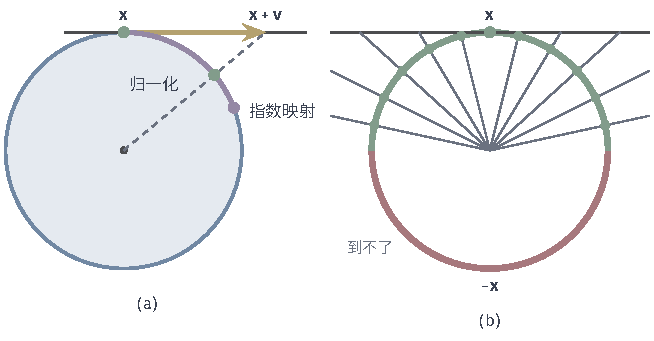
\includegraphics[width=110.8mm]{figures/05-optimization/06-constrained-optimization/tikz/mfo-retraction-cut/figure.pdf}
 \caption{球面的截面。(a)~黄箭头是长度$1.2$的切向量，归一化把它的端点沿虚线径向拉回到绿点，紫弧是指数映射走过的路，端点在紫点。(b)~切线上的点全都被归一化映到上半圆（绿）。下半圆（红）到不了，对跖点$-\bm{x}$也到不了。}
 \label{fig:mfo-retraction-cut}
\end{BookInlineFigure}

两者的差在小步时很小。由$\arctan s=s-s^3/3+O(s^5)$，角度差是$s^3/3$的量级，这是图~\ref{fig:mfo-retraction-error}(b)的斜率$3$。步子大了差距才明显：$s\to\infty$时归一化只能逼近$\pi/2$，而指数映射走过的角度不断增长。

\begin{BookInlineFigure}
 \centering
 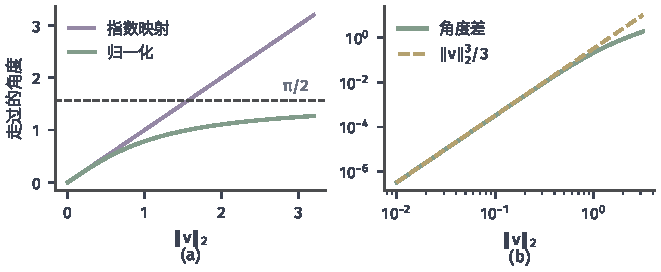
\includegraphics[width=112.0mm]{figures/05-optimization/06-constrained-optimization/matplotlib/mfo-retraction-error/figure.pdf}
 \caption{球面上切向量长度$\lVert\bm{v}\rVert_2$与走过的角度。(a)~指数映射（紫）的角度等于长度，归一化（绿）的角度不超过$\pi/2$。(b)~双对数坐标下两者的角度差（绿）与$\lVert\bm{v}\rVert_2^3/3$（黄虚线）在小步时重合。}
 \label{fig:mfo-retraction-error}
\end{BookInlineFigure}

把切平面整张折到球面上，就看到回缩的全貌。图~\ref{fig:mfo-retraction-grid}中，切平面上等间距的同心圆经过归一化后向边缘挤压，径向的射线变成大圆。这也提醒我们，回缩不是等距的，切空间里的长度只在原点附近才代表流形上走过的距离。

\begin{BookInlineFigure}
 \centering
 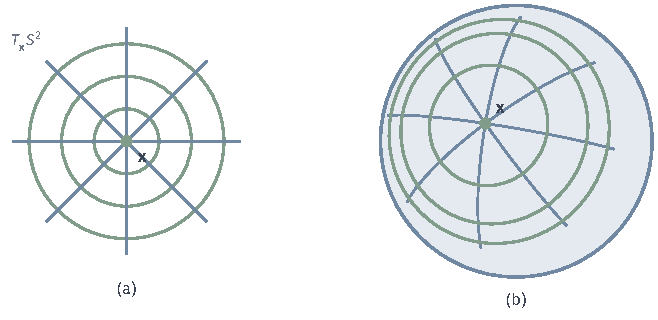
\includegraphics[width=111.3mm]{figures/05-optimization/06-constrained-optimization/tikz/mfo-retraction-grid/figure.pdf}
 \caption{归一化回缩把切平面折到球面上。(a)~切平面上半径$0.5,1,1.5$的同心圆（绿）与八条射线（蓝）。(b)~它们在回缩下的像，同心圆的间距向外收紧，射线变成大圆的一段。}
 \label{fig:mfo-retraction-grid}
\end{BookInlineFigure}

\paragraph{定义域}
归一化公式对所有切向量都有定义，因为$\bm{x}\perp\bm{v}$保证$\bm{x}+\bm{v}\neq\bm{0}$，但它的像只覆盖开上半球，如图~\ref{fig:mfo-retraction-cut}(b)所示。定义~\ref{def:mfo-retraction}只要求在零的邻域内有定义，这对迭代是足够的，因为每步只需要局部信息。

一般回缩可能只在局部有定义，分解还可能有多种选择。选择不固定就会使映射不光滑，下面的矩阵例子就有这个问题。

\paragraph{Stiefel流形上的回缩}
取$\bm{X}\in\mathrm{St}(k,n)$，切向量$\bm{\Delta}$满足$\bm{X}^\top\bm{\Delta}$反对称。把$\bm{X}+\bm{\Delta}$作QR分解$\bm{X}+\bm{\Delta}=\bm{Q}\bm{R}$，其中$\bm{R}$上三角且对角元为正，取$\bm{Q}$作为新点：
\begin{equation}
 R_{\bm{X}}^{\mathrm{QR}}(\bm{\Delta})=\bm{Q}.
 \label{eq:mfo-qr-retraction}
\end{equation}

固定对角元为正这个选择是必要的，否则列的符号可以任意翻转，映射甚至不连续。分解一定存在且唯一，因为$\bm{X}^\top\bm{\Delta}$反对称使两个交叉项抵消：
\[
 (\bm{X}+\bm{\Delta})^\top(\bm{X}+\bm{\Delta})=\bm{I}+\bm{\Delta}^\top\bm{\Delta}\succ\bm{0},
\]
所以$\bm{X}+\bm{\Delta}$列满秩。

下面核对一阶一致性。令$\bm{X}+t\bm{\Delta}=\bm{Q}(t)\bm{R}(t)$，$\bm{Q}(0)=\bm{X}$，$\bm{R}(0)=\bm{I}$。对$t$求导并在$t=0$左乘$\bm{X}^\top$，得到
\[
 \bm{X}^\top\bm{\Delta}=\bm{X}^\top\bm{Q}'(0)+\bm{R}'(0).
\]

左端反对称，右端第一项也反对称（对$\bm{Q}(t)^\top\bm{Q}(t)=\bm{I}$求导得到），所以$\bm{R}'(0)$既反对称又上三角，只能是零。代回求导式就得到$\bm{Q}'(0)=\bm{\Delta}$。

第二种构造用极分解，把$\bm{X}+\bm{\Delta}$的列正交化的同时尽量少动它：
\begin{equation}
 R_{\bm{X}}^{\mathrm{pol}}(\bm{\Delta})=(\bm{X}+\bm{\Delta})\bigl(\bm{I}+\bm{\Delta}^\top\bm{\Delta}\bigr)^{-1/2}.
 \label{eq:mfo-polar-retraction}
\end{equation}

结果确实在流形上：列满秩矩阵右乘$(\bm{Y}^\top\bm{Y})^{-1/2}$后列标准正交。把逆平方根展开，得到
\[
 \bm{C}(t)=(\bm{X}+t\bm{\Delta})\Bigl(\bm{I}-\frac12t^2\bm{\Delta}^\top\bm{\Delta}+O(t^4)\Bigr).
\]
于是$\bm{C}'(0)=\bm{\Delta}$，$\bm{C}''(0)=-\bm{X}\bm{\Delta}^\top\bm{\Delta}$。

后者形如$\bm{X}\bm{B}$，其中$\bm{B}$对称。为了判断它的切向分量，写出$\mathrm{St}(k,n)$的切向投影
\begin{equation}
 \bm{P}_{\bm{X}}(\bm{Z})=\bm{Z}-\bm{X}\operatorname{sym}(\bm{X}^\top\bm{Z}),\qquad \operatorname{sym}(\bm{B})=\frac12(\bm{B}+\bm{B}^\top).
 \label{eq:mfo-stiefel-projection}
\end{equation}
把$\bm{Z}=\bm{X}\bm{B}$代入，得到$\bm{X}\bm{B}-\bm{X}\bm{B}=\bm{0}$，所以极分解回缩是二阶回缩。QR回缩一般只是一阶的，下面的例子中它的加速度有非零的切向分量。

用具体数字比较两种构造。在$\mathrm{St}(2,3)$上取
\[
 \bm{X}=\begin{bmatrix}1&0\\0&1\\0&0\end{bmatrix},\qquad
 \bm{\Delta}=\begin{bmatrix}0&0\\0&0\\1&1\end{bmatrix},\qquad
 \bm{Y}=\bm{X}+\bm{\Delta}=\begin{bmatrix}1&0\\0&1\\1&1\end{bmatrix}.
\]
这里$\bm{X}^\top\bm{\Delta}=\bm{0}$，是切向量。

QR分解按列正交化。第一列除以$\sqrt2$，第二列减去在第一列上的投影再除以长度，于是
\[
 \bm{q}_1=\frac{1}{\sqrt2}(1,0,1)^\top,\qquad
 \bm{q}_2=\frac{1}{\sqrt6}(-1,2,1)^\top.
\]

极分解要用$\bm{I}+\bm{\Delta}^\top\bm{\Delta}$的逆平方根。这个矩阵是
\[
 \bm{I}+\bm{\Delta}^\top\bm{\Delta}=\begin{bmatrix}2&1\\1&2\end{bmatrix},
\]
特征值为$3,1$，特征向量为$(1,1)^\top/\sqrt2$和$(1,-1)^\top/\sqrt2$，算出来的结果是
\[
 R_{\bm{X}}^{\mathrm{pol}}(\bm{\Delta})\approx\begin{bmatrix}0.7887&-0.2113\\-0.2113&0.7887\\0.5774&0.5774\end{bmatrix}.
\]

沿曲线$R_{\bm{X}}(t\bm{\Delta})$算加速度的切向分量，极分解得到零，QR回缩得到
\[
 \bm{P}_{\bm{X}}\bm{C}''(0)=\begin{bmatrix}0&-1\\1&0\\0&0\end{bmatrix},
\]
不是零，这印证了两者阶数的差别。

图~\ref{fig:mfo-stiefel-qr-polar}画出两个结果。QR分解保留第一列的方向，把调整都压给后面的列，极分解则两列对称地调整。两个新点张成同一个平面，这个事实在第~\ref{sec:mfo-representation}节会派上用场。

\begin{BookInlineFigure}
 \centering
 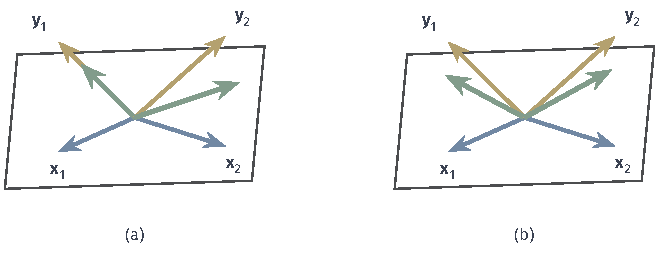
\includegraphics[width=111.6mm]{figures/05-optimization/06-constrained-optimization/tikz/mfo-stiefel-qr-polar/figure.pdf}
 \caption{$\mathrm{St}(2,3)$上的两种回缩。蓝箭头是当前两列，黄箭头是$\bm{X}+\bm{\Delta}$的两列，绿箭头是回缩结果，方框是$\bm{y}_1,\bm{y}_2$张成的平面。(a)~QR分解：第一列方向不变。(b)~极分解：两列对称调整。}
 \label{fig:mfo-stiefel-qr-polar}
\end{BookInlineFigure}

\paragraph{回缩、指数映射与最近点}
第三个候选是把$\bm{x}+\bm{v}$投影到$M$上的最近点。球面上它恰好就是归一化；$\mathrm{St}(k,n)$上在Frobenius范数下恰好就是极分解，例中极分解结果到$\bm{Y}$的距离约为$0.732$，QR结果约为$0.850$。

但回缩并不要求求解最近点问题。QR回缩不是最近点，同样满足定义，而且通常更便宜。在一般曲面上，最近点可能需要迭代才能算出，甚至不唯一。表~\ref{tab:mfo-retraction-compare}比较三者。

\begin{BookInlineTable}
 \centering
 \caption{三种回到流形的方式。“二阶”的结论对最近点投影要求流形足够光滑，表中代价按一次运算计。}
 \label{tab:mfo-retraction-compare}
 \begin{tabular}{llll}
  \toprule
  方式 & 阶 & 球面 & Stiefel\\
  \midrule
  指数映射 & 二阶 & $O(n)$ & 需矩阵指数\\
  最近点投影 & 二阶 & $O(n)$ & 需SVD\\
  QR回缩 & 一阶 & 同归一化 & 约$O(nk^2)$\\
  \bottomrule
 \end{tabular}
\end{BookInlineTable}

\subsection{目标拉回}
\label{sec:mfo-pullback}

\paragraph{把问题搬到同一个切空间}
候选步是切空间中的向量，而目标定义在流形上。把两者复合，就得到切空间上的普通函数，这是后面评价候选步的唯一依据。

\begin{definition}[拉回目标]
 \label{def:mfo-pullback}
 在$\bm{x}\in M$处，目标$f$的\term{拉回}（pullback）是切空间上的函数
 \begin{equation}
  \hat{f}_{\bm{x}}(\bm{v})=f\bigl(R_{\bm{x}}(\bm{v})\bigr),\qquad\bm{v}\in U_{\bm{x}}.
  \label{eq:mfo-pullback}
 \end{equation}
\end{definition}

这个定义的好处是，$\hat{f}_{\bm{x}}$活在线性空间上，前面各章的工具（Taylor展开、Armijo条件、预测下降）都可以直接使用。

贯穿例在$\bm{x}^{(0)}$的切平面上取一组标准正交基：
\[
 \bm{E}_1=\frac13(1,-2,2)^\top,\qquad
 \bm{E}_2=\frac13(2,-1,-2)^\top.
\]
可以检查$\bm{x}^{(0)},\bm{E}_1,\bm{E}_2$两两正交且长度为一。

沿$\bm{v}=s\bm{E}_2$拉回。需要的内积是$\bm{x}^{(0)\top}\bm{A}\bm{E}_2=-\tfrac89$和$\bm{E}_2^\top\bm{A}\bm{E}_2=\tfrac{22}{9}$，代入归一化回缩，得到
\begin{equation}
 \hat{f}_{\bm{x}^{(0)}}(s\bm{E}_2)=\frac{1}{1+s^2}\cdot\frac12\Bigl(\frac{16}{9}-\frac{16}{9}s+\frac{22}{9}s^2\Bigr)=\frac{8-8s+11s^2}{9(1+s^2)}.
 \label{eq:mfo-pullback-line}
\end{equation}

\paragraph{一阶与二阶变化}
下面的引理说明，拉回在零点的一阶信息总是黎曼梯度，二阶信息则取决于回缩的加速度。

\begin{lemma}[拉回的导数]
 \label{lem:mfo-pullback-derivatives}
 设$M$是嵌入子流形，取诱导度量，$R$是回缩，$\bm{v}\in T_{\bm{x}}M$，$\bm{c}(t)=R_{\bm{x}}(t\bm{v})$。则
 \begin{equation}
  \nabla\hat{f}_{\bm{x}}(\bm{0})=\operatorname{grad}f(\bm{x}),
  \label{eq:mfo-pullback-grad}
 \end{equation}
 \begin{equation}
  \langle\bm{v},\nabla^2\hat{f}_{\bm{x}}(\bm{0})\bm{v}\rangle=\langle\bm{v},\operatorname{Hess}f(\bm{x})[\bm{v}]\rangle+\bigl\langle\operatorname{grad}f(\bm{x}),\bm{c}''(0)\bigr\rangle.
  \label{eq:mfo-pullback-hess}
 \end{equation}
\end{lemma}

\begin{proof}
 由复合函数求导和式~\eqref{eq:mfo-retraction-def}，
 \[
  \frac{\mathrm{d}}{\mathrm{d}t}\hat{f}_{\bm{x}}(t\bm{v})\Big|_{t=0}=\mathrm{d}f_{\bm{x}}[\bm{c}'(0)]=\mathrm{d}f_{\bm{x}}[\bm{v}]=\langle\operatorname{grad}f(\bm{x}),\bm{v}\rangle,
 \]
 这是式~\eqref{eq:mfo-pullback-grad}。

 $\hat{f}_{\bm{x}}(t\bm{v})=f(\bm{c}(t))$，把式~\eqref{eq:mfo-second-along-curve}用到曲线$\bm{c}$上，再用式~\eqref{eq:mfo-hess-lagrange}替换第一项，就得到式~\eqref{eq:mfo-pullback-hess}。
\end{proof}

式~\eqref{eq:mfo-pullback-hess}的附加项给出了两条实用的结论。第一，二阶回缩的$\bm{c}''(0)$是法向的，黎曼梯度是切向的，附加项为零，拉回Hessian等于黎曼Hessian。第二，在驻点上$\operatorname{grad}f=\bm{0}$，对任何回缩附加项都为零，所以一般回缩在驻点处两者也相等。

一般回缩在非驻点处可能有差别。圆周的例子最容易看清。取角度$\theta$为坐标，目标
\[
 \varphi(\theta)=\frac12\bigl(\cos^2\theta+4\sin^2\theta\bigr),\qquad
 \varphi'(\theta)=\frac32\sin2\theta,\qquad
 \varphi''(\theta)=3\cos2\theta.
\]

比较三种回缩：指数映射$\theta+s$，归一化$\theta+\arctan s$，以及一个人为构造的一阶回缩$\theta+s+\tfrac12s^2$。第三个满足定义，但沿圆周的加速度是$1$，不是二阶的。对它求拉回的二阶导数，得到
\[
 \hat{f}''(0)=\varphi''(\theta)+\varphi'(\theta).
\]

在$\theta=\pi/6$处，$\varphi'=3\sqrt3/4\approx1.299$，$\varphi''=1.5$。前两种回缩的拉回二阶导数都是$1.5$，第三种是$2.799$。在驻点$\theta=0$处$\varphi'=0$，三者都是$3$。图~\ref{fig:mfo-pullback-curvature}画出这个差别。

\begin{BookInlineFigure}
 \centering
 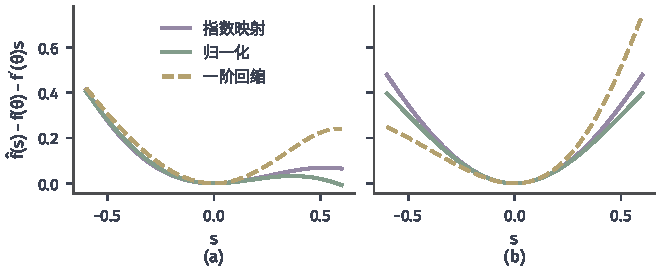
\includegraphics[width=112.0mm]{figures/05-optimization/06-constrained-optimization/matplotlib/mfo-pullback-curvature/figure.pdf}
 \caption{圆周上目标扣除一阶项后的拉回$\hat{f}(s)-\varphi(\theta)-\varphi'(\theta)s$。紫线、绿线、黄虚线分别对应指数映射、归一化与一阶回缩$\theta+s+s^2/2$。(a)~非驻点$\theta=\pi/6$，黄虚线在零点的曲率明显更大。(b)~驻点$\theta=0$，三条曲线在零点处曲率相同。}
 \label{fig:mfo-pullback-curvature}
\end{BookInlineFigure}

\paragraph{用拉回评价候选步}
式~\eqref{eq:mfo-pullback-grad}和式~\eqref{eq:mfo-pullback-hess}支持下面这个切空间二次模型：
\begin{equation}
 m_{\bm{x}}(\bm{v})=f(\bm{x})+\langle\operatorname{grad}f(\bm{x}),\bm{v}\rangle+\frac12\langle\bm{v},\operatorname{Hess}f(\bm{x})[\bm{v}]\rangle.
 \label{eq:mfo-model}
\end{equation}

在贯穿例的方向上核对。沿$s\bm{E}_2$，切向曲率是
\[
 \langle\bm{E}_2,(\bm{A}-q\bm{I})\bm{E}_2\rangle=\frac{22}{9}-\frac{16}{9}=\frac23,
\]
模型是
\[
 m(s\bm{E}_2)=\frac89-\frac89s+\frac13s^2.
\]

用式~\eqref{eq:mfo-pullback-line}减去模型，分子通分后得到
\[
 \hat{f}_{\bm{x}^{(0)}}(s\bm{E}_2)-m(s\bm{E}_2)=\frac{8s^3-3s^4}{9(1+s^2)}.
\]
误差是$s^3$量级，这正是二阶回缩的效果。$s=0.1$时误差约为$8.5\times10^{-4}$，$s=1$时误差是$\tfrac{5}{18}$，模型已不可信，这是信赖域要处理的问题。

\subsection{向量搬运}
\label{sec:mfo-transport}

\paragraph{为什么需要搬运}
共轭梯度要把上一轮的方向和当前梯度相加，拟Newton要算两点梯度之差。欧氏空间里这些都是普通的加减法，流形上却有一个类型错误：旧向量在$T_{\bm{x}}M$中，新向量在$T_{\bm{y}}M$中，两者属于不同的线性空间。

在球面上，不同点的切平面是不同的平面，直接相加得到的向量一般不再切于任何一点。例如$\bm{x}^{(0)}$和$\bm{x}^{(1)}$处的两个切向量之和，通常与$\bm{x}^{(1)}$有非零内积。需要先把旧向量搬到新切空间。

\begin{definition}[向量搬运]
 \label{def:mfo-vector-transport}
 伴随回缩$R$的\term{向量搬运}（vector transport）是一族映射，对$\bm{x}\in M$和$\bm{\eta}\in T_{\bm{x}}M$给出线性映射$\mathcal{T}_{\bm{\eta}}$，它把$T_{\bm{x}}M$映到点$R_{\bm{x}}(\bm{\eta})$的切空间，且随$(\bm{x},\bm{\eta})$光滑变化，并满足$\mathcal{T}_{\bm{0}}=\mathrm{id}$。
\end{definition}

定义只要求三件事：结果落在新切空间中（一致性），对被搬运的向量是线性的，零步时什么也不做。它不要求保持长度和内积。后面需要这些额外性质时，要逐个核对。为了书写简洁，起点$\bm{x}$、终点$\bm{y}=R_{\bm{x}}(\bm{\eta})$明确时，记成$\mathcal{T}_{\bm{x}\to\bm{y}}$。

\paragraph{三种具体搬运}
第一种是\term{投影搬运}（projection transport），把旧向量看作环境空间的向量，投影到新切空间：
\begin{equation}
 \mathcal{T}^{\mathrm{P}}_{\bm{x}\to\bm{y}}(\bm{v})=\bm{P}_{\bm{y}}\bm{v}.
 \label{eq:mfo-projection-transport}
\end{equation}
它只对嵌入子流形可用，计算便宜。正交投影不会增加长度，但一般会减小长度。

第二种是\term{平行移动}（parallel transport），即卷四定义的沿曲线协变导数为零的搬运，它是等距的。球面上沿大圆从$\bm{x}$到$\bm{y}$有闭式：
\begin{equation}
 \mathcal{T}^{\parallel}_{\bm{x}\to\bm{y}}(\bm{v})=\bm{v}-\frac{\langle\bm{x}+\bm{y},\bm{v}\rangle}{1+\langle\bm{x},\bm{y}\rangle}(\bm{x}+\bm{y}).
 \label{eq:mfo-parallel-transport}
\end{equation}
这里要求$\bm{y}\neq-\bm{x}$。

下面验证结果确实切于$\bm{y}$且长度不变。记
\[
 c=\langle\bm{x},\bm{y}\rangle,\qquad a=\langle\bm{x}+\bm{y},\bm{v}\rangle.
\]

由$\bm{v}\perp\bm{x}$有$\langle\bm{y},\bm{v}\rangle=a$，又$\langle\bm{x}+\bm{y},\bm{y}\rangle=1+c$，于是
\[
 \langle\bm{y},\mathcal{T}^{\parallel}\bm{v}\rangle=a-\frac{a}{1+c}(1+c)=0.
\]

再用$\lVert\bm{x}+\bm{y}\rVert_2^2=2+2c$算长度：
\[
 \lVert\mathcal{T}^{\parallel}\bm{v}\rVert_2^2=\lVert\bm{v}\rVert_2^2-\frac{2a^2}{1+c}+\frac{a^2(2+2c)}{(1+c)^2}=\lVert\bm{v}\rVert_2^2.
\]

第三种是\term{微分回缩}（differentiated retraction），直接用回缩曲线的速度：
\[
 \mathcal{T}^{\mathrm{D}}_{\bm{\eta}}(\bm{v})=\frac{\mathrm{d}}{\mathrm{d}t}R_{\bm{x}}(\bm{\eta}+t\bm{v})\Big|_{t=0}.
\]
它的好处是下一节的线搜索导数恰好用这个向量。球面归一化沿搜索方向$\bm{d}$，设$\bm{y}=R_{\bm{x}}(\alpha\bm{d})$，$r=\lVert\bm{x}+\alpha\bm{d}\rVert_2$，求导得到
\[
 \frac{\mathrm{d}}{\mathrm{d}\tau}R_{\bm{x}}\bigl((\alpha+\tau)\bm{d}\bigr)\Big|_{\tau=0}=\frac{1}{r}\bm{P}_{\bm{y}}\bm{d}.
\]
所以此时投影搬运与微分回缩只差一个正的倍数$r$。

\paragraph{搬运结果的比较}
图~\ref{fig:mfo-transport}对比了切向量在两点之间的搬运。把$\bm{v}$平移到$\bm{y}$得到的副本并不切于球面（灰色虚线）。投影把副本垂直压到切平面上，长度变短；平行移动沿大圆旋转切平面，长度不变。

\begin{BookInlineFigure}
 \centering
 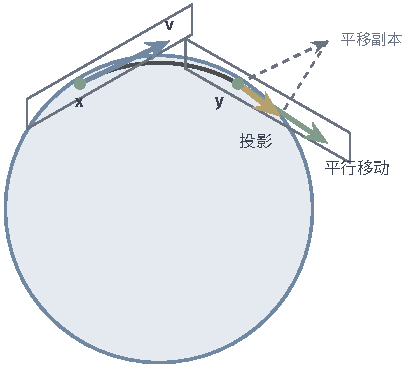
\includegraphics[width=70.0mm]{figures/05-optimization/06-constrained-optimization/tikz/mfo-transport/figure.pdf}
 \caption{把切向量$\bm{v}$（蓝）从$\bm{x}$搬到$\bm{y}$。深灰弧是连接两点的大圆，两个方框是切平面。灰色虚线箭头是平移的副本，不切于球面。黄箭头是投影结果，长度缩短；绿箭头是平行移动结果，长度与$\bm{v}$相同。}
 \label{fig:mfo-transport}
\end{BookInlineFigure}

用贯穿例算一次。第~\ref{sec:mfo-rgd}节将得到$\bm{x}^{(1)}\approx(0.8418,0.5388,-0.0337)^\top$，它与起点的内积约为$0.9091$。把基向量$\bm{E}_1,\bm{E}_2$搬到$\bm{x}^{(1)}$，投影的结果范数约为$0.9949$和$0.9147$，内积约为$0.0408$，平行移动的结果仍是标准正交的。

投影缩短的量取决于向量与连线方向的夹角。沿大圆方向的向量缩短最多，缩短比例等于两点内积。负梯度方向恰好是大圆方向，$\lVert\bm{g}^{(0)}\rVert_2\approx0.9162$的向量投影后长度约为$0.8330$，比值$0.9091$。

因此投影搬运不是等距的：它让向量落进了新切空间，但没有保持内积。若$\bm{y}\perp\bm{x}$，投影还会把沿连线方向的向量压成零，这时映射不可逆。表~\ref{tab:mfo-transport-compare}列出后面的算法需要核对的性质。

\begin{BookInlineTable}
 \centering
 \caption{三种搬运的性质，以球面归一化回缩为例。可逆一栏的$c=\langle\bm{x},\bm{y}\rangle$；一般流形上的平行移动要解常微分方程。}
 \label{tab:mfo-transport-compare}
 \begin{tabular}{llll}
  \toprule
  搬运 & 长度 & 可逆 & 代价\\
  \midrule
  投影 & 一般缩短 & 需$c\neq0$ & $O(n)$\\
  平行移动 & 保持 & 是 & $O(n)$\\
  微分回缩 & 沿步方向缩到$1/r^2$倍 & 需$c\neq0$ & $O(n)$\\
  \bottomrule
 \end{tabular}
\end{BookInlineTable}
